% \documentclass[aspectratio=169,notes]{beamer}
\documentclass[aspectratio=169]{beamer}
\usetheme[faculty=phil]{fibeamer}
\usepackage{polyglossia}
\setmainlanguage{english} %% main locale instead of `english`, you
%% can typeset the presentation in either Czech or Slovak,
%% respectively.
\setotherlanguages{russian} %% The additional keys allow
%%
%%   \begin{otherlanguage}{czech}   ... \end{otherlanguage}
%%   \begin{otherlanguage}{slovak}  ... \end{otherlanguage}
%%
%% These macros specify information about the presentation
\title[Artificial Intelligence Software (AIS)]{Artificial Intelligence Software, Lecture 1} %% that will be typeset on the
\subtitle{Introduction  
\\ Intro to MLOps \\ \  } %% title page.
\author{Oleg Bulichev}
%% These additional packages are used within the document:
\usepackage{ragged2e}  % `\justifying` text
\usepackage{booktabs}  % Tables
\usepackage{tabularx}
\usepackage{tikz}      % Diagrams
\usetikzlibrary{calc, shapes, backgrounds}
\usetikzlibrary{decorations.pathreplacing,calligraphy,calc,graphs}
\usepackage{amsmath, amssymb}
\usepackage{url}       % `\url`s
\usepackage{listings}  % Code listings
% \usepackage{subfigure}
\usepackage{floatrow}
\usepackage{subcaption}
\usepackage{mathtools}
\usepackage{todonotes}
\usepackage{fontspec}
\usepackage{multicol}
\usepackage{pdfpages}
\usepackage{wrapfig}
\usepackage{qrcode}
\usepackage{animate}
\usepackage{booktabs}
\usepackage{multirow}
% \usepackage{graphicx}
\usepackage{colortbl}

\graphicspath{{resources/}}
\frenchspacing

\setbeamertemplate{caption}[numbered]
\usetikzlibrary{graphs}

% \usepackage[backend=biber,style=ieee,autocite=footnote]{biblatex}
% \addbibresource{biblio.bib}
% \DefineBibliographyStrings{english}{%
%   bibliography = {References},}

\newcommand{\oleg}[2][] {\todo[color=red, #1] {OLEG:\\ #2}}
\newcommand{\fbckg}[1]{\usebackgroundtemplate{\includegraphics[width=\paperwidth]{#1}}}%frame background

\usepackage[framemethod=TikZ]{mdframed}
\newcommand{\dbox}[1]{
\begin{mdframed}[roundcorner=3pt, backgroundcolor=yellow, linewidth=0]
\vspace{1mm}
{#1}
\vspace{1mm}
\end{mdframed}
}

\begin{document}
\setlength{\abovedisplayskip}{0pt}
\setlength{\belowdisplayskip}{0pt}
\setlength{\abovedisplayshortskip}{0pt}
\setlength{\belowdisplayshortskip}{0pt}

\fbckg{fibeamer/figs/title_page.png}
\frame[c]{\setcounter{framenumber}{0}
    \usebeamerfont{title}%
    \usebeamercolor[fg]{title}%
    \begin{minipage}[b][6.5\baselineskip][b]{\textwidth}%
        \textcolor{black}{\raggedright\inserttitle}
    \end{minipage}
    % \vskip-1.5\baselineskip

    \usebeamerfont{subtitle}%
    \usebeamercolor[fg]{framesubtitle}%
    \begin{minipage}[b][3\baselineskip][b]{\textwidth}
        \raggedright%
        \insertsubtitle%
    \end{minipage}
    \vskip.25\baselineskip
}
%   \frame[c]{\maketitle}

\fbckg{fibeamer/figs/common.png}

\note{\scriptsize \begin{itemize}
        \item \
    \end{itemize}}

\begin{frame}[t]{About Me (1)}
    \framesubtitle{}
    \begin{columns}[T,onlytextwidth]
        \begin{column}{0.49\textwidth}
            \begin{figure}[H]
                \centering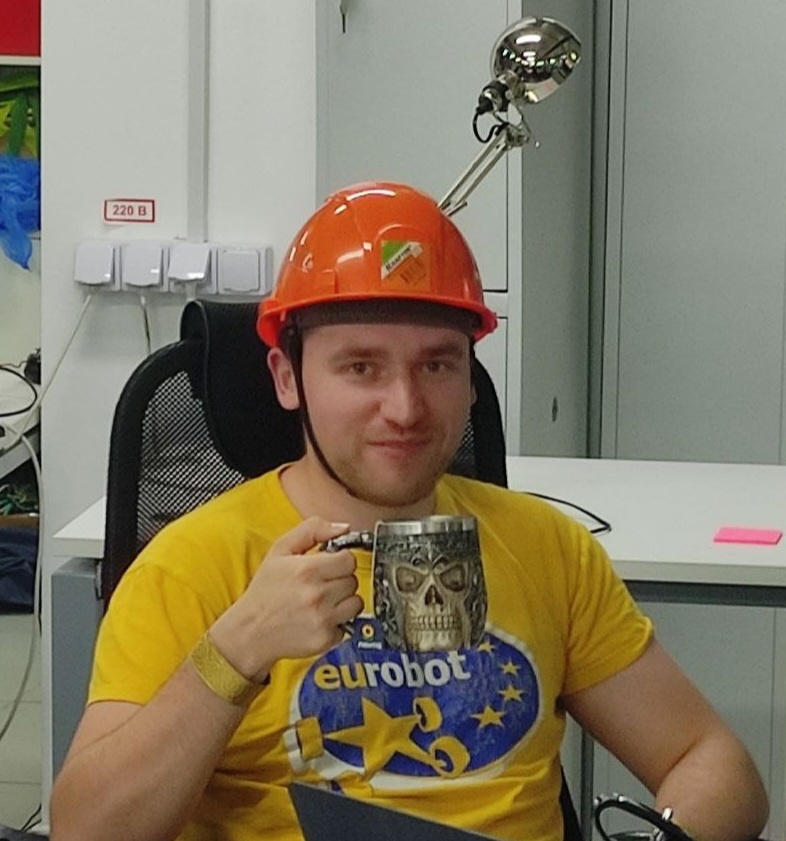
\includegraphics[height=5cm,width=1\textwidth,keepaspectratio]{Oleg.jpg}
                % \caption{caption_name}
                \label{fig:Oleg.jpg}
            \end{figure}
        \end{column}
        \begin{column}{0.49\textwidth}
            \Large
            \vspace{2cm}
            \centering
            \textbf{PhD Oleg Bulichev} \\
            \textit{Mail}: \url{bulichev.ov@mipt.ru}\\
            \textit{TG}: \url{@Lupasic} \\
            \textit{Office Hours}: By request
        \end{column}
    \end{columns}
\end{frame}

\begin{frame}[t]{About Me (2)}
    \framesubtitle{}
    \begin{columns}[T,onlytextwidth]
        \begin{column}{0.69\textwidth}
            \textbf{Education}
            \begin{itemize}
                \item \textit{Bachelor} --- BMSTU (МГТУ им Н.Э. Баумана) <<CAD developer>>
                \item \textit{Master \& PHD} --- Innopolis University (IU) <<Robotics>>
            \end{itemize}
            \textbf{Job}
            \begin{itemize}
                \item \textit{Lead Engineer, Senior Research Fellow} --- MIPT, Center for Cognitive Modeling: SLAM and robotics hardware development
                \item \textit{Associate Professor} --- IU: Supervisor
            \end{itemize}
        \end{column}
        \begin{column}{0.29\textwidth}
            \begin{figure}[H]
                \centering
                \qrcode[height=3cm]{https://t.me/WildOlegAdventures} % Generates a QR code for the link
                \caption*{\textbf{Link to my channel}}
                \label{fig:qrcode}
            \end{figure}
        \end{column}
    \end{columns}
\end{frame}

\begin{frame}[c]{Course Goal}
    \framesubtitle{}
    \centering \Large
    To obtain an \textbf{instrumental foundation} (the \textbf{tools}) \\
    so that in subsequent courses \\
    (Intro to ML, DL, RL, etc.) \\
    \medskip
    \textit{you can learn to \textbf{build a house}}
\end{frame}

\begin{frame}[t]{Course puprose and objectives}
    \framesubtitle{}
    Our laboratory works with \textbf{AI in its full scope}, with special attention to \textbf{robotics}. 
    
    Therefore, it's important for us to:
    \begin{itemize}
        \item Not only find solutions as \textbf{researchers}
        \item But also \textbf{maintain} and \textbf{deploy} them to hardware competently
        \item Create \textbf{demos and web interfaces} with running models for presentations
    \end{itemize}
    \medskip
    
    We will go through the \textbf{complete pipeline} and learn its various \textbf{tools}:
    \begin{multicols}{2}
        \begin{itemize}
            \item \textbf{Data Management}
            \item \textbf{Model Selection \& Configuration}
            \item \textbf{Training \& Monitoring}
            \item \textbf{Demo Development}
            \item \textbf{Optimization \& Deployment}
            \item \textbf{Robotics tools}
        \end{itemize}
    \end{multicols}
\end{frame}

\begin{frame}[t]{Course challenges}
\framesubtitle{}
    \begin{itemize}
        \item Inverse education (first tools, then theory)
        \item A lot of coding and debugging
        \item Dive into the "jungle" of tools and frameworks
        \item Completely new course
    \end{itemize}
\end{frame}

\begin{frame}[t]{Course outline and organization}
    \framesubtitle{}
    % \vspace{-0.6cm}
    Three big blocks:
    \begin{itemize}
        \item Tools: Conda, Docker, VibeCoding, Literature Review using AI, ROS (Robotics Operating System), Simulators
        \item Training pipeline: Data management, Model selection, Training and monitoring
        \item Deployment pipeline: Demo development, Model optimization, Deployment to hardware
    \end{itemize}
\end{frame}

\begin{frame}[t]{Grading criteria}
    \framesubtitle{}
    \begin{columns}[T,onlytextwidth]
        \begin{column}{0.49\textwidth}
            \textbf{What will be evaluated on the course}
            \begin{itemize}
                \item[Qz:] Quizzes: $4\times 5=20\%$ 
                \item[HWs:] Homework assignments: $40\%$
                \item[CP:] Course project: $2\times 15=30\%$
                \item[FE:] Final Exam: $10\%$
                \item[Extra:] Slide fixes in Github: $5\%$ 
            \end{itemize}
        \end{column}
        \begin{column}{0.49\textwidth}
            \textbf{Late policy:} -50\% of max grade for a task \\
            \textbf{Scale}:
            \begin{itemize}
                \item[5:] 85 --- 100\%
                \item[4:] 70 --- 84.99\%
                \item[3:] 50 --- 69.99\%
                \item[2:] 0 --- 49.99\% or less than $50\%$ by any criterion. 
            \end{itemize}
        \end{column}
    \end{columns}
\end{frame}

\begin{frame}[t]{Quizzes}
    \framesubtitle{}
        \textbf{Purpose}: Quizzes help us to understand what you didn't get during the previous lecture.
        \bigskip

    \textbf{Format}: $5-15\ min$ closed book on a paper sheet, in the beginning of a lecture. \\
    \end{frame}

\begin{frame}[t]{Course Project}
    \framesubtitle{}
    Projects are extended version of homeworks.

    \textit{Idea for project 1:} Build a custom image classifier for 5-10 classes, deploy it on a web server with a simple web interface.
    \medskip

    \textit{Idea for project 2:} Take pre-trained YOLO, label your data, fine-tune, deploy on PC, integrate your camera with robotics simulator.
\end{frame}

\begin{frame}[c]{}
    \framesubtitle{}
    \centering \LARGE \textbf{Lab Goals} \\
    To obtain the needed tools for solving the design part of the competition
\end{frame}

\begin{frame}[c]{}
    \framesubtitle{}
    \centering\LARGE
    \textbf{Agreements among the group (for now)}
\end{frame}

\begin{frame}[t]{Pretest}
    \framesubtitle{}
    \LARGE
    \begin{multicols}{2}
        \begin{itemize}
            \item Dataset
            \item Model
            \item Training
            \item Inference
            \item Deployment
            \item Pipeline
        \end{itemize}
    \end{multicols}
\end{frame}

\begin{frame}[t]{Key Terms (1/2)}
    \framesubtitle{}
    \begin{itemize}
        \item \textbf{Dataset}: Collection of data used to train or test models
        \\ \textit{Example: ImageNet, KITTI}
        
        \item \textbf{Model}: Mathematical representation that learns patterns from data
        \\ \textit{Example: YOLO, ResNet}
        
        \item \textbf{Training}: Process of teaching a model by feeding it data
        \\ \textit{Example: Using PyTorch to adjust model weights}
    \end{itemize}
\end{frame}

\begin{frame}[t]{Key Terms (2/2)}
    \framesubtitle{}
    \begin{itemize}
        \item \textbf{Inference}: Using a trained model to make predictions on new data
        \\ \textit{Example: Running YOLO to detect objects in a video stream}
        
        \item \textbf{Deployment}: Making a model available for use in production
        \\ \textit{Example: Hosting model on a server, deploying to Jetson}
        
        \item \textbf{Pipeline}: Automated sequence of steps from data to deployment
        \\ \textit{Example: Data $\rightarrow$ Training $\rightarrow$ Testing $\rightarrow$ Deployment}
    \end{itemize}
\end{frame}

\begin{frame}{}
\framesubtitle{}
    \centering \LARGE Let's discuss ML pipelines you used/heard before!
\end{frame}


\begin{frame}[t]{Pipeline Overview}
    \framesubtitle{}
    \centering
    \begin{tikzpicture}[
        node distance=1.5cm,
        every node/.style={
            rectangle, 
            rounded corners, 
            minimum width=2.4cm, 
            minimum height=1cm,
            text centered, 
            draw=black, 
            fill=blue!10,
            font=\footnotesize
        },
        arrow/.style={thick,->,>=stealth}
    ]

    % Top Row
    \node (data) [fill=green!10] {Data Lifecycle};
    \node (model) [right of=data, xshift=2.2cm] {Model Selection};
    \node (train) [right of=model, xshift=2.2cm] {Training};
    \node (eval) [right of=train, xshift=2.2cm] {Evaluation};

    % Bottom Row
    \node (opt) [below of=train, yshift=-1.5cm] {Optimization};
    \node (dep) [left of=opt, xshift=-2.2cm] {Deployment};
    \node (mon) [left of=dep, xshift=-2.2cm] {Monitoring};

    % Arrows
    \draw [arrow] (data) -- (model);
    \draw [arrow] (model) -- (train);
    \draw [arrow] (train) -- (eval);
    \draw [arrow] (eval) |- (opt);
    \draw [arrow] (opt) -- (dep);
    \draw [arrow] (dep) -- (mon);
    \draw [arrow] (mon) -- ++(-1.8,0) |- (data);

    \end{tikzpicture}
\end{frame}

\begin{frame}[t]{1. Data Lifecycle}
    \framesubtitle{Garbage in, garbage out} 
    \begin{itemize}
        \item \textbf{Key Steps}: Collection, Annotation (Labeling), Versioning
        \item \textbf{Why it's needed}: A model cannot learn what isn't in the data. Reproducible data ensures reproducible results.
        \item \textbf{Example Task}: Collecting video from a robot, drawing bounding boxes around obstacles, creating a Dataset v1.0 snapshot.
    \end{itemize}
\end{frame}

\begin{frame}[t]{2. Model Selection}
    \framesubtitle{Don't reinvent the wheel}
    \begin{itemize}
        \item \textbf{Key Steps}: Literature review, Selecting pre-trained architectures, Configuring hyperparameters.
        \item \textbf{Why it's needed}: Starting from a pre-trained model (SOTA) saves weeks of compute time and resources.
        \item \textbf{Example Task}: Choosing a lightweight object detector that works well on a small dataset of traffic signs.
    \end{itemize}
\end{frame}

\begin{frame}[t]{3. Training}
    \framesubtitle{Scientific approach to experiments}
    \begin{itemize}
        \item \textbf{Key Steps}: Fine-tuning, Logging metrics/weights, Hyperparameter optimization.
        \item \textbf{Why it's needed}: To understand \textit{which} change improved the model and to be able to reproduce the best result.
        \item \textbf{Example Task}: Running 10 experiments with different learning rates and selecting the one with the lowest loss curve.
    \end{itemize}
\end{frame}

\begin{frame}[t]{4. Evaluation}
    \framesubtitle{Proof of Concept (PoC)}
    \begin{itemize}
        \item \textbf{Key Steps}: Calculating metrics (IoU, Accuracy on test set), Visual testing (Demo UI).
        \item \textbf{Why it's needed}: Dry metrics don't always reflect reality. Stakeholders need to "see" how it works on real examples.
        \item \textbf{Example Task}: Creating a simple web interface where you upload a photo and see the robot's planned path.
    \end{itemize}
\end{frame}

\begin{frame}[t]{5. Optimization}
    \framesubtitle{Making it fit the hardware}
    \begin{itemize}
        \item \textbf{Key Steps}: Format conversion, Quantization (e.g. FP32 $\rightarrow$ INT8), Hardware compilation.
        \item \textbf{Why it's needed}: Python is often too slow for real-time robotics. Robots have limited battery and compute power.
        \item \textbf{Example Task}: Reducing model size by 4x to run at 30 FPS on a robot's onboard computer.
    \end{itemize}
\end{frame}

\begin{frame}[t]{6. Deployment}
    \framesubtitle{Integrating the brain into the body}
    \begin{itemize}
        \item \textbf{Key Steps}: Containerization, Inference Server setup, Hardware integration.
        \item \textbf{Why it's needed}: To run the model reliably in a production environment (outside the developer's laptop), handling errors and restarts.
        \item \textbf{Example Task}: Packaging the model into a container that automatically starts when the robot turns on.
    \end{itemize}
\end{frame}

\begin{frame}[t]{7. Monitoring}
    \framesubtitle{The world changes, and so should the model}
    \begin{itemize}
        \item \textbf{Key Steps}: Metric collection, Alerting, Data Drift detection.
        \item \textbf{Why it's needed}: To know when the model starts failing (e.g., at night, in snow, or due to sensor degradation) \textit{before} users complain.
        \item \textbf{Example Task}: A dashboard showing that the confidence of obstacle detection drops significantly during rain.
    \end{itemize}
\end{frame}

\begin{frame}[t]{Is this pipeline universal?}
    \framesubtitle{ML, DL, NLP, CV, RL ... ?}
    \begin{itemize}
        \item Does the \textbf{Data $\rightarrow$ Model $\rightarrow$ Deploy} cycle apply to all AI fields?
        \item \textbf{Yes!} The high-level stages remain the same.
        \item \textbf{However}, the tools, data formats, and specific challenges ("bottlenecks") differ significantly.
        \item Key domains we will touch: \textbf{Classical ML}, \textbf{Computer Vision (CV)}, \textbf{NLP}, \textbf{Reinforcement Learning (RL)}.
    \end{itemize}
\end{frame}

\begin{frame}[t]{Classical ML}
    \framesubtitle{Structured Data, Spreadsheets, SQL}
    \begin{itemize}
        \item \textbf{Data}: Structured (rows/columns). Feature Engineering is crucial (handling missing values, normalization).
        \item \textbf{Model}: Light architectures (Random Forest, XGBoost, Linear Regression).
        \item \textbf{Pipeline Specifics}:
            \begin{itemize}
                \item Training is fast (minutes/seconds).
                \item Explainability is easier (Feature Importance).
                \item Deployment is lightweight (often just a serialized pickle file).
            \end{itemize}
        \item \textbf{Example}: Bank credit scoring, Customer churn prediction.
    \end{itemize}
\end{frame}

\begin{frame}[t]{Computer Vision (CV) \& NLP}
    \framesubtitle{Unstructured Data (Deep Learning)}
    \begin{itemize}
        \item \textbf{Data}: Images, Video, Text, Audio. Requires huge storage and specialized labeling (bounding boxes, tokens).
        \item \textbf{Model}: Deep Neural Networks (CNNs, Transformers).
        \item \textbf{Pipeline Specifics}:
            \begin{itemize}
                \item Needs GPUs for training (hours/days).
                \item Data Augmentation is key.
                \item Transfer Learning (Pre-trained models) is standard.
            \end{itemize}
        \item \textbf{Example}: Face recognition, ChatGPT, Object Detection.
    \end{itemize}
\end{frame}

\begin{frame}[t]{Reinforcement Learning (RL)}
    \framesubtitle{The Outlier: Learning by Interaction}
    \begin{itemize}
        \item \textbf{Data}: Not a static dataset! Data is generated by the Agent interacting with an Environment (Simulation).
        \item \textbf{Model}: Policy Networks (Agents).
        \item \textbf{Pipeline Specifics}:
            \begin{itemize}
                \item "Training" loop involves simulation steps (millions of frames).
                \item \textbf{Sim2Real gap}: Hard to transfer from simulation to reality.
                \item Reward Engineering instead of Labeling.
            \end{itemize}
        \item \textbf{Example}: Robot walking, AlphaGo, Dota 2 bots.
    \end{itemize}
\end{frame}

\begin{frame}[t]{Reference Materials}
    \framesubtitle{}
    TODO
    % \begin{enumerate}
    %     \item \href{https://werk24.io/knowledge-base-technical-drawings/title-block}{Title Block}
    %     \item \href{https://thepresentation.ru/grafika/vvedenie-metody-proetsirovaniya-tochka-proetsirovanie-tochki}{Методы проецирования (RUS)}
    %     \item \href{https://studfile.net/preview/3366860/page:6/}{Инженерная графика (RUS)}
    % \end{enumerate}
\end{frame}


\fbckg{fibeamer/figs/last_page.png}
\frame[plain]{}

\end{document}